\documentclass[conference]{IEEEtran}
\usepackage[T1]{fontenc}
\usepackage{graphicx}
\usepackage{amsmath}
\usepackage{booktabs}
\usepackage{url}
\usepackage[hidelinks]{hyperref}
\title{Simple Digital Image Processing Techniques and Suitable Features for Three Practical Cases}
\author{\IEEEauthorblockN{Student Name}
\IEEEauthorblockA{Digital Image Processing Course\\University / Department}}
\begin{document}
\maketitle
\begin{abstract}
Digital image processing can solve practical problems without requiring complex machine-learning models. This report examines three introductory cases: counting coins, enhancing a scanned document, and removing impulse noise from a photograph. For each case, a simple processing pipeline is implemented and the image features supporting that pipeline are identified. The accompanying Python notebook uses publicly accessible sample images and produces all reported figures and measurements. Global thresholding detects 21 objects against a manual reference of 24 coins, illustrating the limitations of a basic segmentation baseline. Local thresholding reduces the document's foreground fraction from 35.68\% to 14.77\%, although this is not an accuracy measurement. For the simulated noise experiment, a median filter improves peak signal-to-noise ratio from 17.77 to 30.12 dB. These examples show that useful features depend on the task, image conditions, and evaluation method.
\end{abstract}
\begin{IEEEkeywords}
digital image processing, feature selection, thresholding, connected components, median filtering
\end{IEEEkeywords}

\section{Introduction}
Digital image processing transforms an image into a more useful representation or extracts information from its pixels. Typical applications include automatic counting, document preparation, and image restoration. A suitable technique should be chosen from the properties of the problem rather than from its complexity. For example, a coin's area may be useful for counting objects, but it does not directly explain how to remove noise from a photograph.

This report considers three cases that are practical for an introductory course. The goals are to summarize each problem, identify appropriate features, implement understandable methods, and discuss actual results and limitations. The implementation uses NumPy, Matplotlib, and scikit-image, a documented Python image-processing library~\cite{skimage2014}. No training data, neural network, or graphics processing unit is required.

\section{Data and Experimental Procedure}
Three images from the official scikit-image collection are used~\cite{samples}: \texttt{coins} ($303\times384$ pixels), \texttt{page} ($191\times384$), and \texttt{camera} ($512\times512$). The collection was located through a web search and the samples were obtained through the original library, rather than downloading untraceable search-engine thumbnails. Coins are credited to the Brooklyn Museum collection with no known copyright restrictions; the current camera image is CC0 by Lav Varshney. The scanned page is supplied by scikit-image without a separately identified photographer in its API entry; no separate public-domain claim is made for it. The repository retains source links and the upstream license notice.

All images are converted to floating-point grayscale values in $[0,1]$. The notebook records package versions, saves the original images, exports comparison figures, and writes measurements to a JSON file. Parameters are fixed for these examples, not optimized on a held-out dataset. The noise experiment uses NumPy's random generator with seed 42. The results are therefore small demonstrations, not evidence of performance across a population of images.

\section{Case I: Counting Coins}
\subsection{Problem and Suitable Features}
Counting visible objects is useful in inventory inspection and simple automation. Here, the task is to count separated coins on a relatively dark background, not to recognize their monetary value. Grayscale intensity provides an initial foreground/background cue. Connected-component area helps remove tiny regions, while the centroid gives each detected object's location. Circularity describes how closely a component resembles a circle:
\begin{equation}
C=\frac{4\pi A}{P^2},
\end{equation}
where $A$ is area and $P$ is perimeter. An ideal continuous circle has $C=1$; discrete boundaries and segmentation errors affect the measured value. Circularity is exported as a descriptive feature, not used as an additional rejection threshold in this baseline.

\subsection{Processing Method}
The image is smoothed with a Gaussian filter of standard deviation 1 pixel. Otsu's method selects a global threshold by separating gray-level classes~\cite{otsu1979}. Pixels above the threshold are treated as foreground. Regions smaller than 120 pixels are removed and holes below 120 pixels are filled. Components touching the image border are discarded, after which connected components are labeled. Each remaining label is counted as one candidate coin. These area settings are specific to the current image resolution.

\begin{figure}[t]
\centering
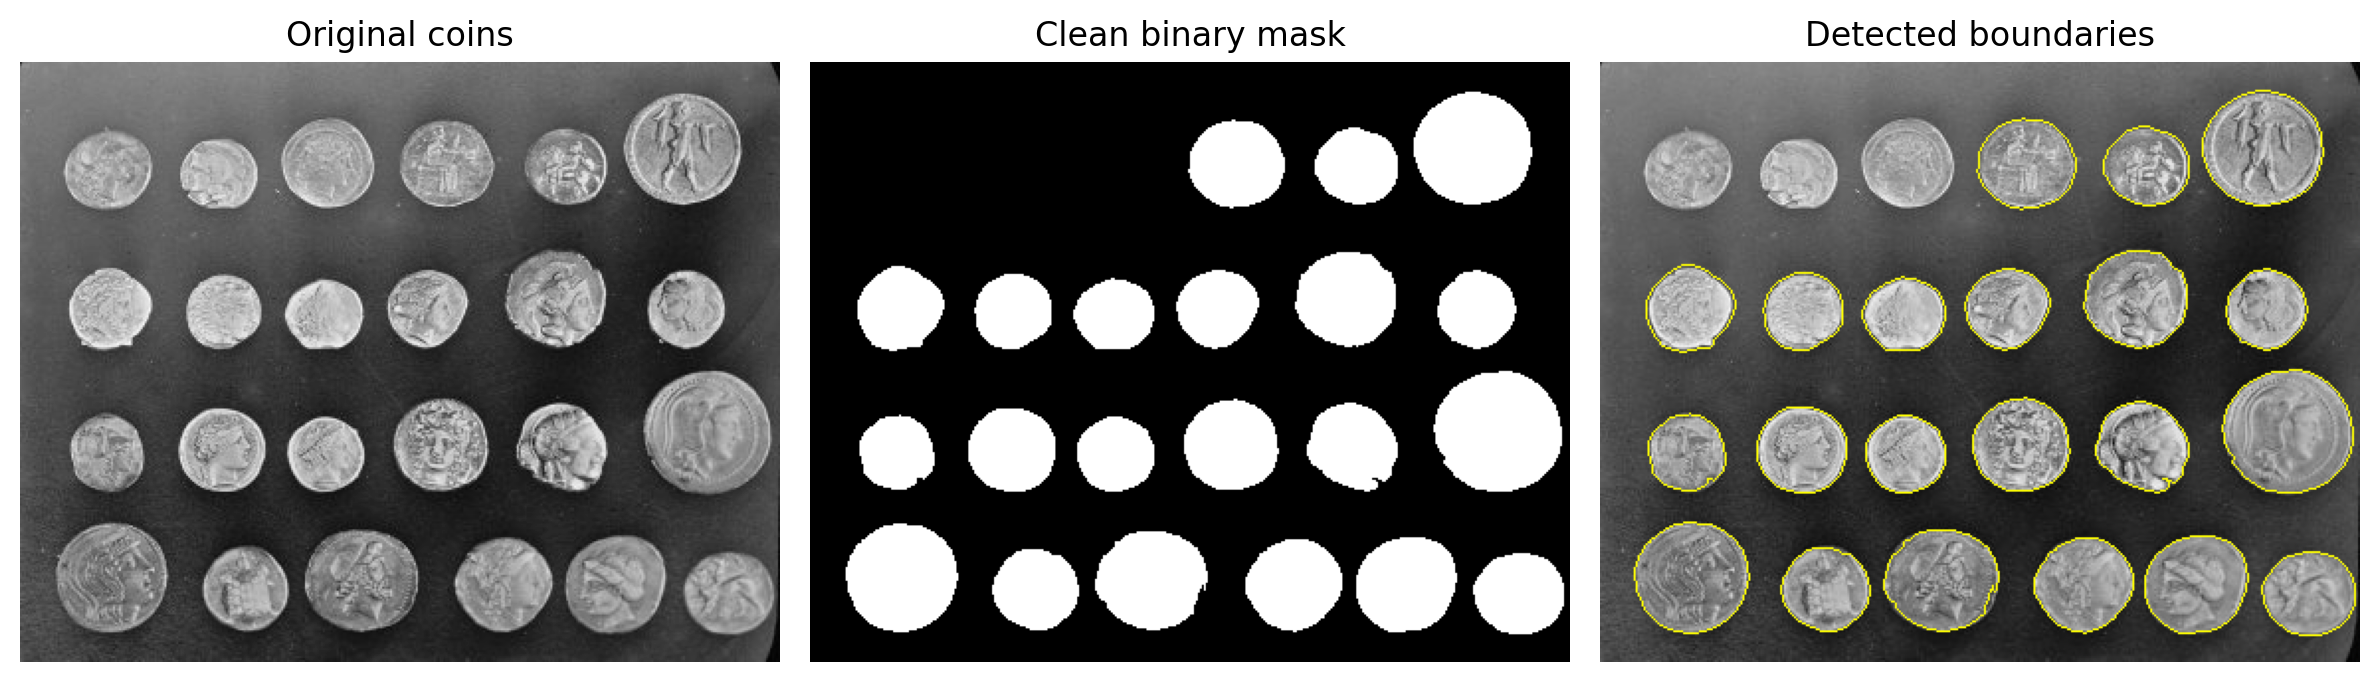
\includegraphics[width=\columnwidth]{figures/coins_results.png}
\caption{Coin-counting baseline: original image, cleaned foreground mask, and detected boundaries. Bright background areas complicate global thresholding.}
\label{fig:coins}
\end{figure}

\subsection{Results and Limitations}
The measured threshold is 0.4073 and the method returns 21 objects. A manual count of the original image gives 24 coins, so the absolute count error is 3 and the relative count error is $3/24=12.5\%$. This is a count discrepancy, not a precision, recall, or object-detection accuracy score. The mask in Fig.~\ref{fig:coins} shows why a global threshold is imperfect: some upper coins are connected to bright background regions that are subsequently removed by border clearing.

The baseline is useful because its failure can be explained. Uneven illumination violates the assumption of separable foreground intensities. Touching coins could also produce one component instead of two, and genuine edge objects would be removed by border clearing. An improved exercise could try local segmentation or watershed separation, but these are not necessary to understand the current introductory pipeline. A reliable system would need annotated object masks or centers across many images.

\section{Case II: Enhancing a Scanned Document}
\subsection{Problem and Suitable Features}
Scanned documents often have shadows or uneven illumination that make fixed thresholding unreliable. The goal is to separate dark text from paper before a possible optical character recognition (OCR) step. Relevant features are local intensity, local contrast, connected-component size, and the fraction of pixels marked as text. Local features are appropriate because the brightness of the paper varies spatially.

\subsection{Processing Method}
Two binarization methods are compared: a single global Otsu threshold and a spatially varying Gaussian-weighted threshold~\cite{thresholds}. The local method uses a $35\times35$ neighborhood and an offset of 0.03:
\begin{equation}
T(x,y)=\mu_w(x,y)-0.03,
\end{equation}
where $\mu_w$ is the weighted local mean. A pixel is marked as text when $I(x,y)<T(x,y)$. The binary results are displayed with black text on a white background. The text fraction is calculated directly from the foreground mask, before display inversion.

\begin{figure}[t]
\centering
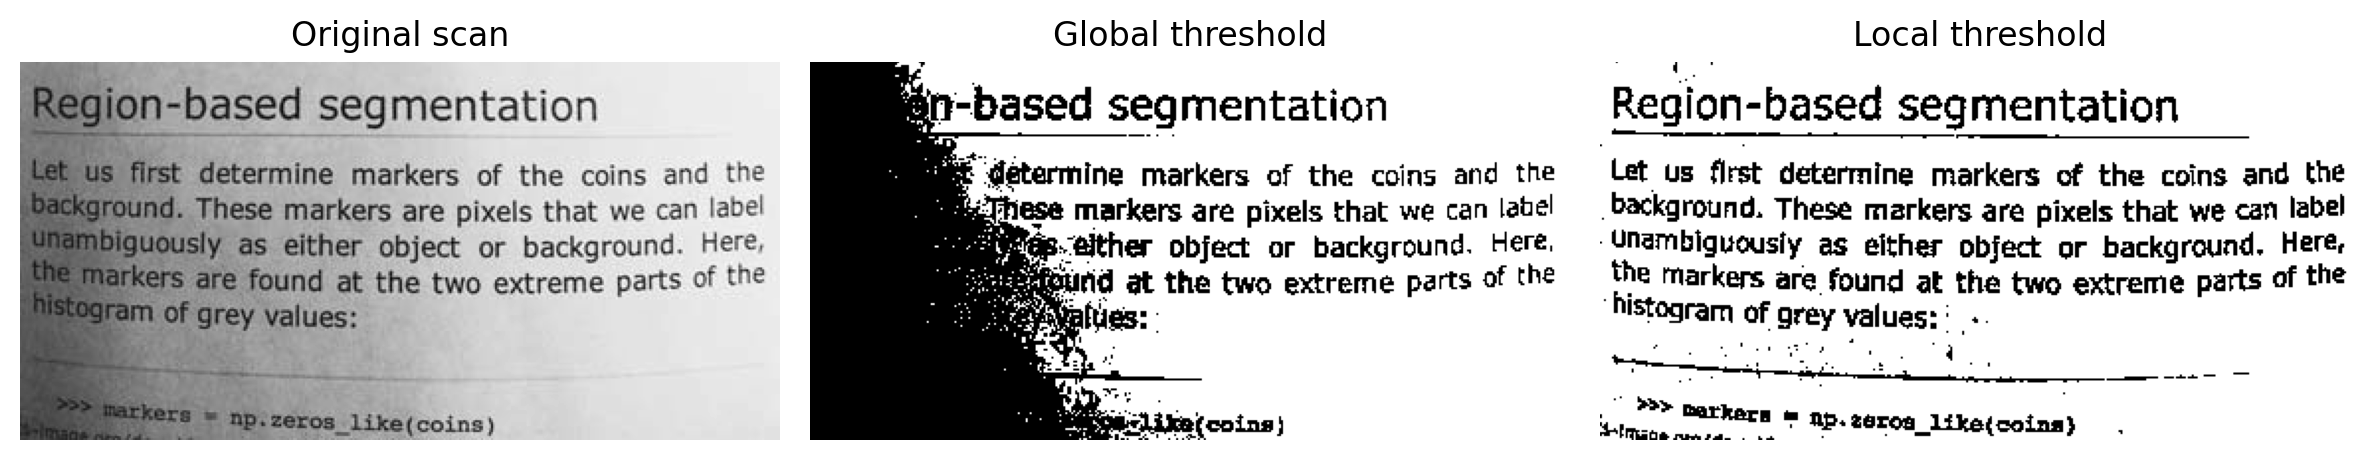
\includegraphics[width=\columnwidth]{figures/document_results.png}
\caption{Document enhancement: original scan, global thresholding, and local thresholding. A spatially varying threshold better follows the background brightness in this example.}
\label{fig:document}
\end{figure}

\subsection{Results and Limitations}
The foreground fraction changes from 35.68\% with the global method to 14.77\% with the local method. The local mask contains 291 connected components, with a median area of 35 pixels. Visual inspection of Fig.~\ref{fig:document} supports the interpretation that local thresholding rejects more of the shaded background while retaining much of the printed text.

However, a lower foreground fraction does not prove better recognition: lost letters also reduce that fraction. Connected components are not equivalent to characters because dots, punctuation, and joined strokes form separate or merged regions. No ground-truth binary mask or transcription is supplied, so pixel accuracy and OCR accuracy are not reported. Important failure cases include thin strokes, textured paper, and text larger than the chosen neighborhood. Practical evaluation should measure character or word error rates on transcribed pages, in addition to inspecting the image.

\section{Case III: Removing Impulse Noise}
\subsection{Problem and Suitable Features}
Impulse corruption introduces isolated black and white pixels, sometimes called salt-and-pepper noise. Extreme intensity and disagreement with neighboring pixels are useful cues. The neighborhood median is an appropriate local statistic because it is less affected by isolated extremes than an arithmetic average. This task therefore uses local intensity consistency rather than object shape.

\subsection{Processing and Evaluation}
For each clean-image pixel, a uniform random value is generated. Values below 0.025 set the pixel to black and values above 0.975 set it to white, giving an expected corruption proportion of 5\%. The original image remains available as a reference. A Gaussian filter with standard deviation 1 pixel and a median filter with a $3\times3$ footprint are applied to the same noisy image.

For $N$ pixels, mean squared error and peak signal-to-noise ratio are
\begin{align}
\mathrm{MSE}&=\frac{1}{N}\sum_{i=1}^{N}(I_i-\hat I_i)^2,\\
\mathrm{PSNR}&=10\log_{10}\!\left(\frac{1}{\mathrm{MSE}}\right),
\end{align}
where $I$ is the clean reference and $\hat I$ is the tested image. The peak value is 1 because the intensity range is normalized. These reference-based metrics evaluate restoration; they are not features available to a real filter when the clean image is unknown.

\begin{table}[t]
\caption{Measured Restoration Results for One Image and Seed}
\label{tab:noise}
\centering
\begin{tabular}{lrr}
\toprule
Image & MSE & PSNR (dB)\\
\midrule
Noisy input & 0.016707 & 17.77\\
Gaussian filtered & 0.002704 & 25.68\\
Median filtered & 0.000973 & 30.12\\
\bottomrule
\end{tabular}
\end{table}

\begin{figure}[t]
\centering
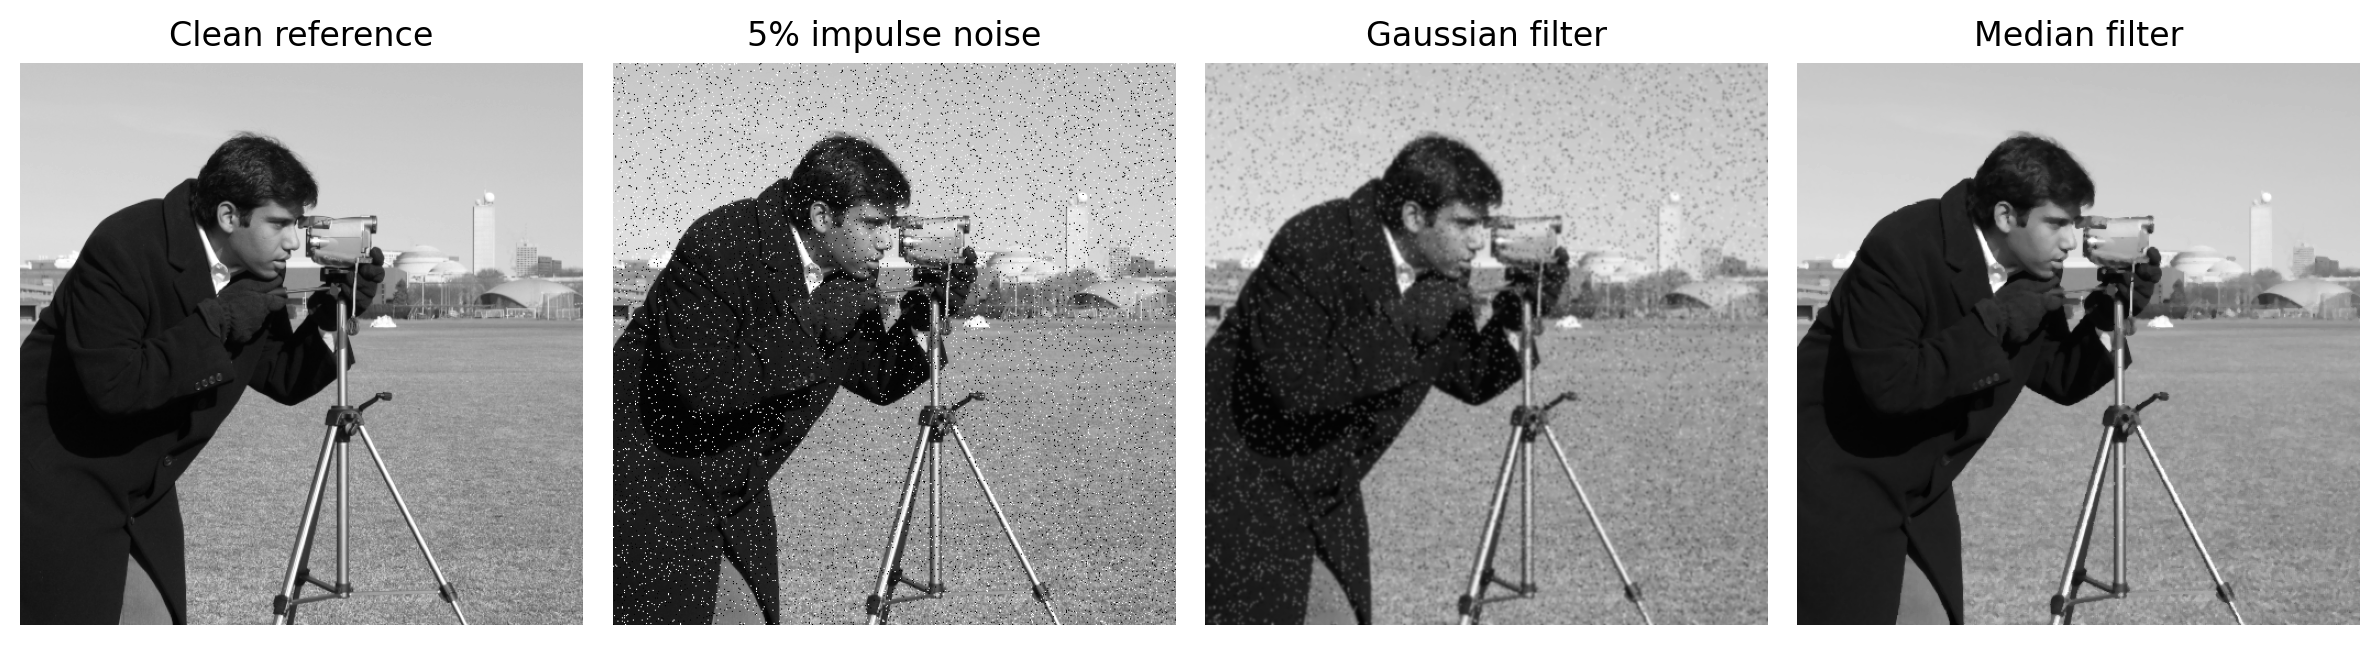
\includegraphics[width=\columnwidth]{figures/denoising_results.png}
\caption{Clean reference, simulated impulse noise, Gaussian-filter output, and median-filter output. Median filtering rejects isolated extremes but can smooth fine details.}
\label{fig:noise}
\end{figure}

\subsection{Results and Limitations}
Table~\ref{tab:noise} shows that median filtering provides the lowest MSE and highest PSNR in this controlled experiment. Its PSNR improvement over the noisy image is 12.35 dB, compared with 7.91 dB for Gaussian filtering. This agrees with the noise model: averaging spreads extreme values into nearby pixels, while the median can reject isolated outliers. Fig.~\ref{fig:noise} provides a qualitative comparison.

Both filters can remove small details. Dense impulses can overwhelm the median, and Gaussian filtering may be more appropriate for a different noise distribution. The numerical ranking applies only to the tested image, corruption model, parameters, and seed. In real photographs, a clean reference is usually unavailable; no-reference inspection or a separate controlled test set would then be needed.

\section{Discussion: Matching Features to the Task}
The three cases illustrate distinct feature roles. In coin counting, intensity creates candidate regions and geometric features describe them. In document enhancement, local brightness and contrast support pixel classification, while component size and text fraction provide diagnostics. In denoising, neighborhood statistics guide restoration and reference errors quantify its outcome. A diagnostic statistic should not be confused with an accuracy score or an inference-time feature.

The simplest method is not always the most accurate, but it is useful when its assumptions and errors are visible. Image scale, illumination, noise type, and object overlap all affect parameter choices. A fair extension would include more samples, annotated references where appropriate, and parameter selection on different data from the final evaluation set. The notebook deliberately keeps these distinctions explicit instead of presenting a successful-looking output as proof of general reliability.

\section{Conclusion}
Three accessible image-processing pipelines were implemented using basic operations. Intensity and geometry support coin counting, local contrast supports document binarization, and neighborhood statistics support impulse-noise removal. The experiments demonstrate both usefulness and limitations: coin counting underestimates the reference, document statistics require cautious interpretation, and median filtering performs well for the simulated impulse model. Selecting features that match the physical problem is more important than choosing an unnecessarily advanced algorithm. The accompanying executable notebook and saved measurements make these introductory observations reproducible.

\bibliographystyle{IEEEtran}
\bibliography{references}
\end{document}
